\begin{surferIntroPage}{Simple Singularities}{simplesing_A1pm}{Simple Singularities}
This gallery visualizes the most important class of singularities of algebraic surfaces, the so--called Simple or ADE--Singularities.

An (algebraic) surface is the set of points $p=(x_0, y_0, z_0)$ in real $3$--space (imagine the three--dimensional space in which we live) which satisfies an equation $f(x_0, y_0, z_0)=0$. Here $f(x,y,z)$ is a polynomial in three variables $x,y,z$, that is a sum of terms (i.e. products of the variables with real numbers as coefficients), such as $x^2+y^2-z^2$ or $x^2+y^2+z^2+2xyz-1$ or $x^3+x^2y^2-3y^2$. The biggest sum of the exponents of a term of $f$ is called its degree (which is $2$, resp. $3$, resp. $4$ in the above examples).

The simplest example of a surface is a plane, given by an equation (of degree $1$)
\[ ax+by+cz-d=0
\]
where $a,b,c,d$ are real numbers ($a, b, c$ not all $0$). The next simple surface is a sphere (of radius $1$) given by
\[
x^2+y^2+z^2-1=0
\]
or, more generally, an ellipsoid with equation $(x/a)^2+(y/b)^2+(z/c)^2-1=0$ (of degree $2$) with $a,b,c$ real numbers.

These surfaces are non--singular or smooth, that is, they look locally in a neighbourhood of each point like a plane, e.g. they do not have any apex or self--intersection or pieces meeting tangentially.

Non--smooth points are called singular or singularities. Formally a singular point $p=(x_0, y_0, z_0)$ of a surface given by $f(x,y,z)=0$ satisfies $f(x_0, y_0, z_0)=0$ (i.e. $p$ is a point of the surface) and all partial derivatives of $f$ satisfy $\partial f/\partial x (x_0, y_0, z_0)=\partial f/\partial y (x_0, y_0, z_0)=\partial f/\partial z(x_0, y_0, z_0)=0$. The simplest singularity is the point $p=(0,0,0)$ of the surface $x^2+y^2-z^2=0$, the double cone (or ordinary double point or $A_1$--singularity).

 Examples of smooth surfaces are a sphere or a torus (the first 2
    pictures), examples of singular surfaces are $A_1, A_2, A_3$ (the last 3 pictures): 
    \begin{center}
      \vspace{-0.2cm}
      \begin{tabular}{@{}c@{}c@{}c@{\quad}c@{}c@{}c@{}c@{}}
        \begin{tabular}{@{}c@{}}
          smooth:
        \end{tabular}
        &
        \begin{tabular}{@{}c@{}}
          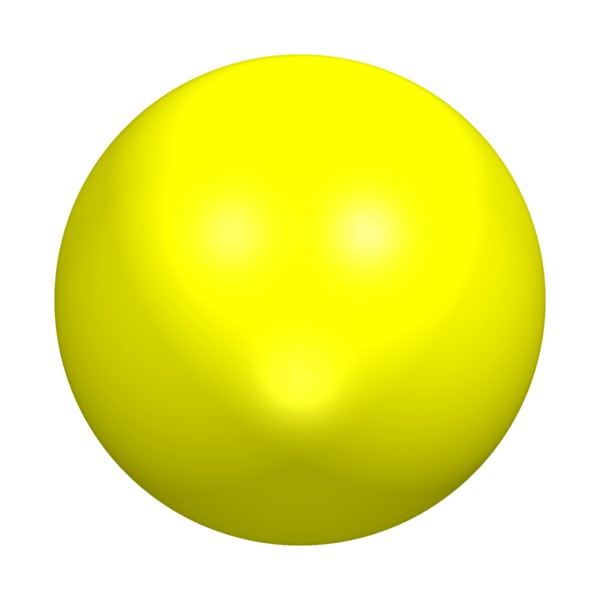
\includegraphics[width=1.1cm]{../../common/images/kugel}
        \end{tabular}
        &
        \begin{tabular}{@{}c@{}}
          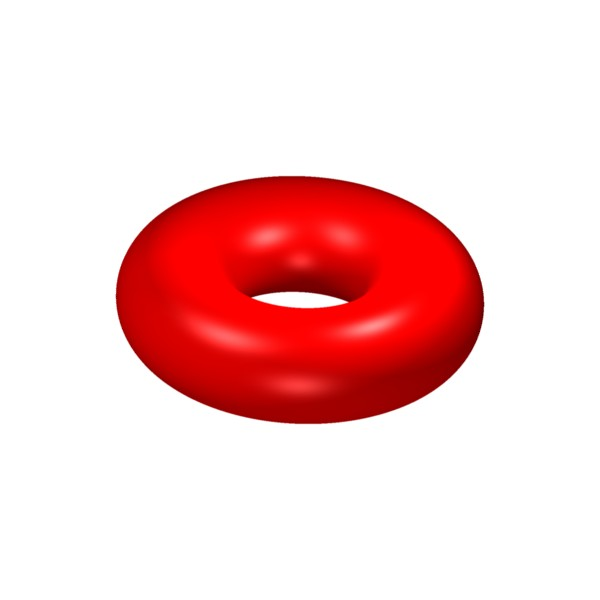
\includegraphics[width=1.1cm]{../../common/images/torus}
        \end{tabular}
        &
        \begin{tabular}{@{}c@{}}
          singular:
        \end{tabular}
        &
        \begin{tabular}{c@{}@{}}
          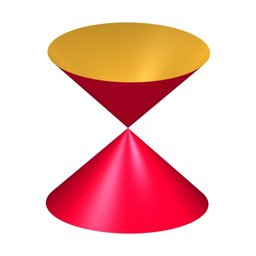
\includegraphics[width=1.1cm]{../../common/images/kegel}
        \end{tabular}
        &
        \begin{tabular}{c@{}@{}}
          \includegraphics[width=1.1cm]{../../common/images/A2pm}
        \end{tabular}
        &
        \begin{tabular}{c@{}@{}}
          \includegraphics[width=1.1cm]{../../common/images/A3pm_0}
        \end{tabular}
      \end{tabular}
    \end{center}
    \vspace{-0.2cm}
    
The Simple or ADE--Singularities are given by the two infinite series of equations
\[
\begin{array}{lll}
A_k^{\pm\pm}: & x^{k+1}\pm y^2\pm z^2=0, & k>1\\
D_k^{\pm\pm}: & x^{k-1}\pm x^2y\pm z^2=0, & k\geq 4
\end{array}
\]
and the three (''exceptional'') singularities
\[
\begin{array}{ll}
E^\pm_0: & x^3\pm y^4\pm z^2=0\\
E^\pm_7: & x^3\pm xy^3\pm z^2=0\\
E^\pm_8: & x^3\pm y^5\pm z^2=0
\end{array}
\]
The ADE--Singularities are in a sense the simplest singularities.


    The rightmost picture above shows an $A_3^{+-}$ singularity (blue), the
    magenta surface is of type $A_2^{+-}$, and the red one of type $A_1^{+-}$
    (\emph{double cone}).
    
The importance of these singularities is due to the fact tat they have amazing relations to numerous different areas of mathematics (their names come from relation to the simple Lie groups of the same name), to mathematical physics and to real life (e.g. in geometric optics). Not all of these relations are fully understood.

Using the Surfer everyone can visualize these singularities. However, the complexity cannot be directly seen from their picture. A better way is to deform the equation slightly (in a special way) and to visualize the deformed surface. This is the purpose of this gallery.


    One can prove that each $A_k$-singularity can be deformed into $\lfloor\frac{k+1}{2}\rfloor$
    $A_1$-singularities; for an $A_3^{+-}$, we obtain two $A_1^{+-}$ (see
    three pictures on the left):
%    \dontshow{
    % 
    \begin{center}
      \vspace{-0.2cm}
      \begin{tabular}{@{}c@{\quad}c@{}c@{\qquad\quad}c@{\quad}c@{\quad}c@{}}
        \begin{tabular}{@{}c@{}}
          \includegraphics[width=1.2cm]{../../common/images/A3pm_0}
        \end{tabular}
        &
        \begin{tabular}{@{}c@{}}
          \includegraphics[width=1.2cm]{../../common/images/A3pm_1}
        \end{tabular}
        &
        \begin{tabular}{@{}c@{}}
          \includegraphics[width=1.2cm]{../../common/images/A3pm_2}
        \end{tabular}
        &
        \begin{tabular}{@{}c@{}}
          \includegraphics[width=1.2cm]{../../common/images/A3pm_vz_2}
        \end{tabular}
        &
        \begin{tabular}{@{}c@{}}
          \includegraphics[width=1.2cm]{../../common/images/A3pm_vz_1}
        \end{tabular}
        &
        \begin{tabular}{@{}c@{}}
          \includegraphics[width=1.2cm]{../../common/images/A3pm_vz_0}
        \end{tabular}
      \end{tabular}
      \\
      \begin{tabular}{@{}c@{\qquad\qquad}c@{}}
          $A_3 \qquad\quad \rightarrow \qquad 2 A_1$
          &
          $2$ Zykel $+$ $1$ Zykel \ $\rightarrow \ A_3$
        \end{tabular}
    \end{center}
%    }
    \vspace*{-0.2cm}
    The index $k$ of the $A_k$--singularities is the so--called \emph{Milnor
      Number} of the singularity; this is the number of \emph{vanishing
      cycles} of the singularity, i.e.\ the number of \emph{holes} which vanish when
    contracting them to the singular point (see pictures on the right). 

For a deeper understanding of these singularities one needs actually complex numbers, i.e. the points $(x_0, y_0, z_0)$ of the ''surface'' $f(x,y,z)=0$ lie in complex $3$--spaces (real $6$--space), bus this cannot be visualized.
\end{surferIntroPage}
